\documentclass[main.tex]{subfiles}
% \nomenclature[A]{GPR}{Ground Penetrating Radar}%

\begin{document}
\chapter{Testing}
\chaplabel{testing}
Tests were conducted to ensure that each subsystem was functioning correctly. Quad bike testing included initial testing of electronic components with subsequent stages added for total system integration to ensure that the autonomous navigation objective was complete. Sensor tests included initial testing to identify sensitivities of the frequency, material properties and soil types. Further tests were completed to identify output metrics and verify the signal processing algorithm developed. 
%%%%(\textcolor{red}{Need to explain testing for GPR and metal detector and integrated systems testing})

\section{Test plan ???}
\textcolor{red}{Maz wants a new section that explains why we are doing the tests we are doing, and what the structure of the overall test plan is. \textbf{Within each subsequent section, start with aims of test, cover the test plan/requirements (need to include schematics and tables), discuss the results and talk about the relevance to the project objectives}}

%%%%%%%%%%%%%%%%%%%%%%%%%%%
\todo[inline]{Rac (Sensors) and Peter (Quad bike) to explain}
%%%%%%%%%%%%%%%%%%%%%%%%%%%

A test plan was completed and attached in Appendix H. This test plan includes specific objectives of the tests for the quad bike platform and two sensors, AMDS metal detector and SIROPULSE II GPR. The quad bike test objectives outlines the requirement to ensure functionality of the modified actuators and sensors and to test the navigation software on the real platform. The sensor suite test objective is to gather data in order to verify sensitivities of the frequency, material properties and soil type, and foremost the signal processing algorithm outlines in detailed design. 

The test plan outlines the required resources to complete the objectives and describes the environment and set-up required for the quad bike and the sensors. It also discusses who is responsible for the tests and additional documentation required to record test data. 

\section{Sensor testing}
The completed tests and its procedure is discussed and includes details of the target objects buried and scanned with the AMDS metal detector and SIROPULSE II GPR. The results from these tests are provided with further analysis of the limitations and how the data is used. 

\subsection{Test procedure}
\seclabel{testProcedure}
The purpose of sensor testing was to confirm that the algorithm produced in the detailed design section functioned correctly, and to gather further data points in order to build up a database for target identification. The testing plan outlined in (\Chapref{testProcedureApp}) provides detailed information regarding the overall goals and objectives for each test completed and the procedures for testing with the two sensors. 

\Figref{testlane} shows the schematic of the test grid that landmines and clutter objects were buried. The target objects were scanned forwards from the APM to the AT and back six times to produce 12 sets of data. 

\begin{figure}[ht]
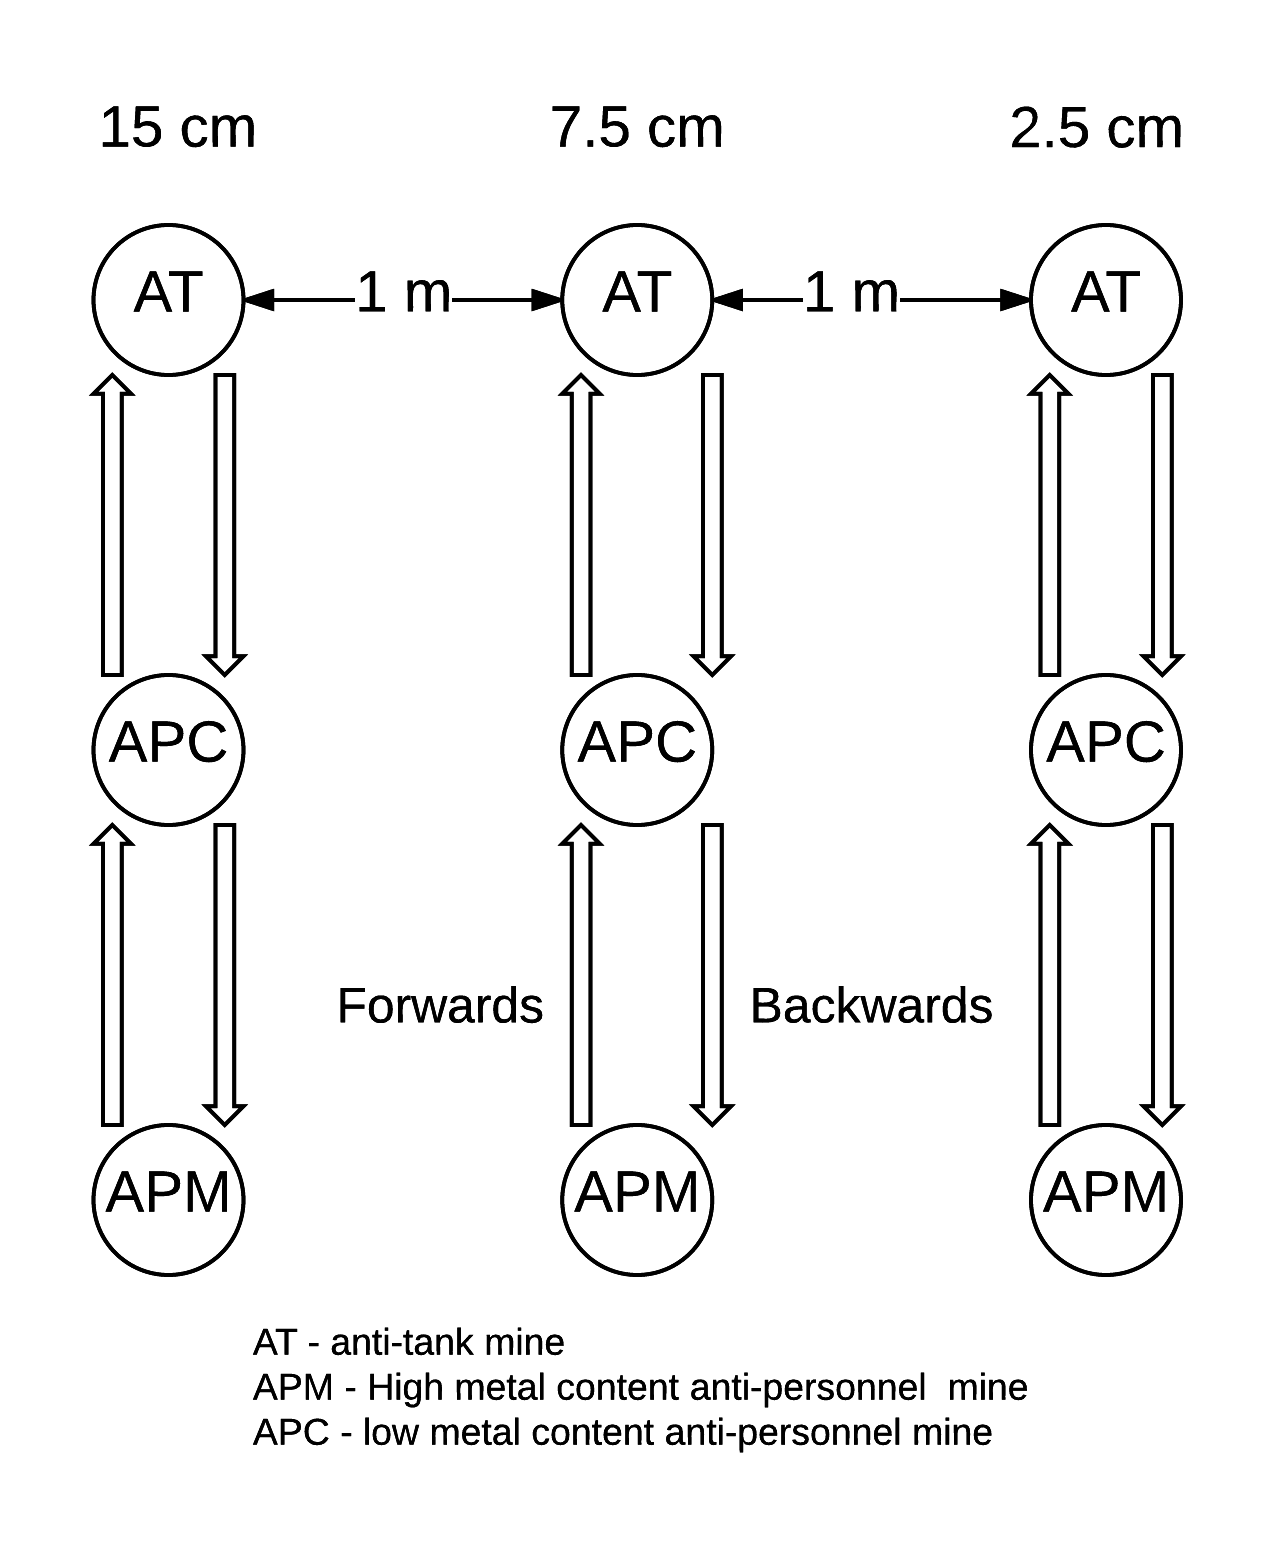
\includegraphics[width=0.6\textwidth]{5-Testing/testlane.png}
\centering
\caption[Schematic of test grid]{Schematic of the test grid where landmines and clutter objects were buried}
\figlabel{testlane}
\end{figure}

In order to identify landmine signatures, replica (dummy) landmines loaned from the DSTG were used. These dummy landmines have similar characteristics to real landmines, including size, material composition and density. The three dummy landmines used were an metallic anti-tank mine (AT), a high metal content anti-personnel mine (APM) and a low metal content anti-personnel mines (APC) as seen in \Figref{dummy}. The APM contains greater than 10 grams of metal, and the APC contains less than 10 grams of metal \parencite{chant2005dsto}. The insides of the replica landmines are filled with paraffin wax and nylon to simulate the properties of real landmines when used with electromagnetic induction equipment \parencite{chant2005dsto}. These landmines are expected to have a density between 1.6 to 1.8 g/cm$^3$, whereas, the soil is expected to have a density between 1.0 to 2.5 g/cm$^3$ \parencite{das2002soil}.		
\begin{figure}[ht]
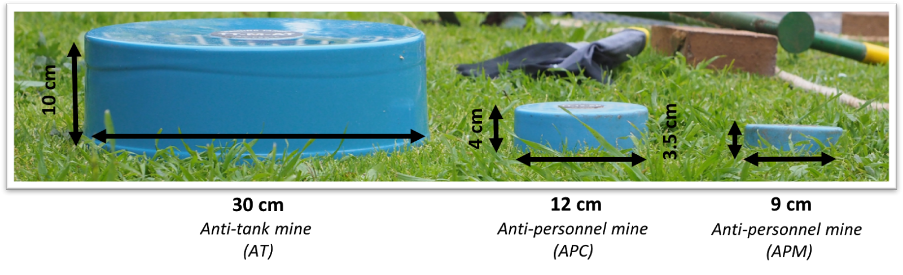
\includegraphics[width=0.9\textwidth]{5-Testing/dummy.PNG}
\centering
\caption{Landmine replicas used for testing }
\figlabel{dummy}
\end{figure}

The dummy landmines were compared to several clutter objects present, representing false positives that could be found in conflict areas. The clutter objects used in the test are shown in \Figref{clutter}. These can be categorised as metallic (steel, aluminium, tin, lead) and non-metallic content (rocks, plastic, wood). Some of these objects were used as they were expected to have similar properties and signatures to real landmines. Identifying these objects using both sensors and producing the metrics defined in detailed design will then lead to a quantifiable range of outputs to classify both dummy landmines and clutter objects.

\begin{figure}[ht]
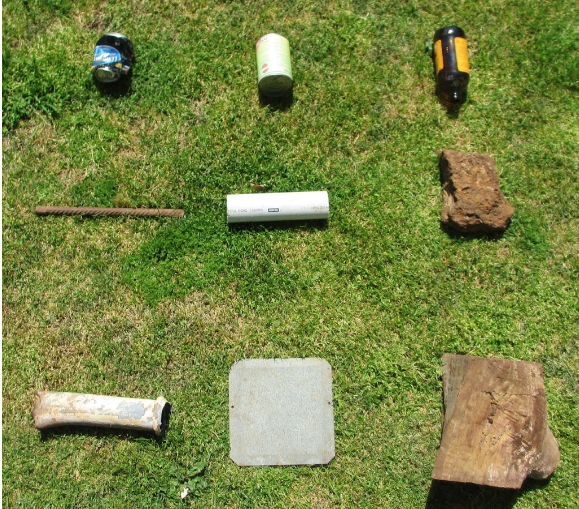
\includegraphics[width=0.6\textwidth]{5-Testing/clutter.PNG}
\centering
\caption[Clutter objects buried in the ground]{Clutter objects buried in the ground, from top left to bottom right: aluminium, tin can, glass bottle, steel rebar, pvc pipe, large rock, lead pipe, galvanised metal plate and wooden stump}
\figlabel{clutter}
\end{figure}

The dummy landmines were buried at three different depths, 2.5 cm, 7.5 cm and 15 cm respectively as shown in \Figref{testlane}, as these depths are used by the DSTG in their standardised landmine detection test procedures. The depths are used to identify and compare the strength of the reflected signals for both metal detector and GPR as landmines are buried at varying depths. The clutter objects were buried at only 7.5 cm depth for an average comparison between the two depths. 

The central transmission frequency of 1.4 GHz was selected for the GPR antennae head. This frequency was found to provide a balance between detection depth and signal resolution and increase signal to noise ratio in comparison to both 800 MHz and 2 GHz GPR antennae. Data was recorded at all four available frequencies for the metal detector.

The testing was completed by scanning over each target column in the grid 12 times, six forwards and six backwards in order to produce large dataset. The data from both metal detector and ground penetrating radar were collected and processed with the algorithms defined in the detailed design chapter. Discussion and analysis of the results from the test is provided in the next section. 

\subsection{Results}
Analysis of the results from the main test will enable confirmation of unique metrics for both metal detector and ground penetrating radar. Feature analysis will be completed independently due to the different output metrics produced by the different signals. 

\subsubsection{Metal detector}
The phase angle and signal magnitude are the two main characteristics that were investigated. The metal detector data processed was analysed based on the magnitude and phase angle variation with target depth, and the phase angle variation versus the signal magnitude.

\Figref{phaseDepth} shows the phase angle result of the objects at varying depths. It is found that the phase angle is consistent across the three operating depths, as expected based on the results of the completed outdoor preliminary tests. The average phase angle for both anti-tank and high metal content anti-personnel mine were positive 25 degrees and negative 50 degrees, respectively. From the nine clutter objects tested, only five signatures may be compared with these two landmines. Based on the calculated results, the only object with phase angles closely similar to the anti-tank mine is the thin galvanised plate with an average phase angle of positive 16 degrees. However, the plate’s signature is differentiable from the actual anti-tank mine using the second metric. 
\begin{figure}[ht]
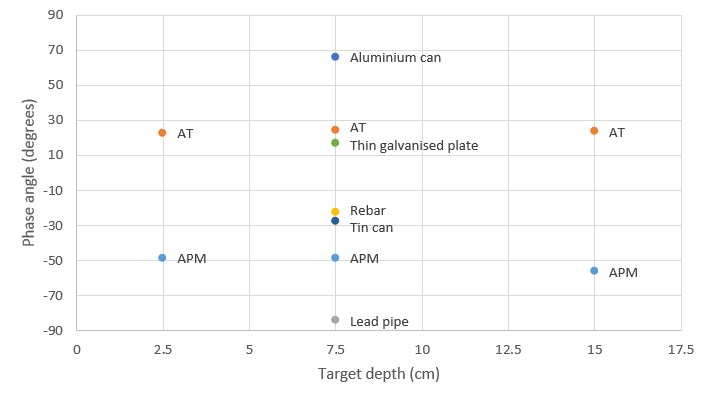
\includegraphics[width=\textwidth]{5-Testing/phaseDepth.PNG}
\centering
\caption{Phase angle variation with target depth }
\figlabel{phaseDepth}
\end{figure}

Upon inspection of the graph (\Figref{magDepth}), signal magnitude with varying depths, the two landmines provide distinguishable magnitudes when compared with the other clutter objects. This graph also confirms that there is a differentiation between the anti-tank mine and the thin galvanised plate. This information can then be used to increase the probability of detection between these two objects. 

The anti-personnel mine and steel rebar have two similar signatures, with an average signal magnitude of 7.9e4 and 6.9e4, respectively. This factor provides an increase in false positive detection rate for the anti-personnel mine if they are both detected simultaneously. However, this false positive detection rate is reduced by analysing the phase angle of the object shown in the previous \Figref{phaseDepth}.

\begin{figure}[!ht]
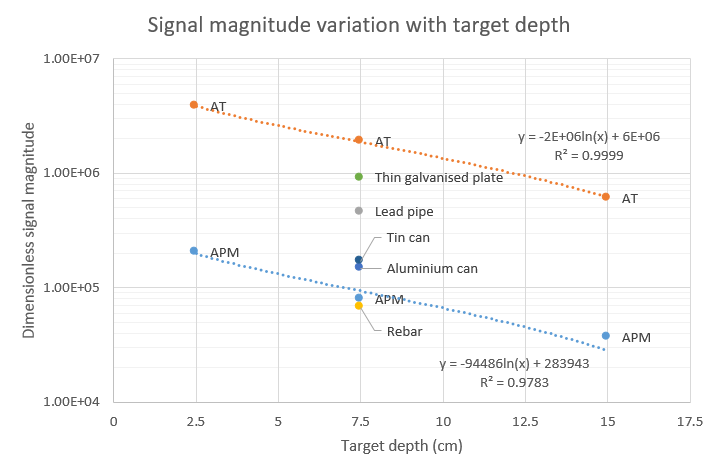
\includegraphics[width=\textwidth]{5-Testing/magDepth.PNG}
\centering
\caption{Signal magnitude variation with target depth }
\figlabel{magDepth}
\end{figure}

When the phase angle is plotted against the signal magnitude (\Figref{phaseMag}), it was found that the phase angle calculated was consistent with a variation in magnitude of signals and thus, can be deduced that the phase angle is independent of the depth or magnitude. From this point, a confidence interval may be given to a phase angle value and confirmed with the corresponding signal magnitude range. 

A noticeable result for this plot is that the thin galvanised plate was within the signatures of the anti-tank mines. This means that it may be detected by the metal detector as an anti-tank mine and increase the false positive rate. 

\begin{figure}[ht]
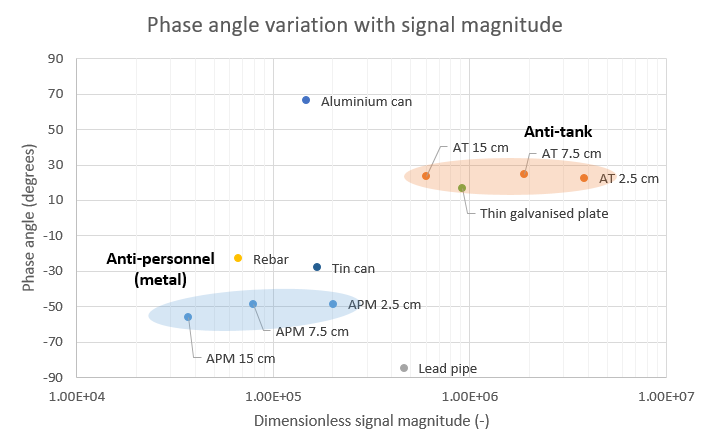
\includegraphics[width=\textwidth]{5-Testing/phaseMag.PNG}
\centering
\caption{Phase angle variation with signal magnitude}
\figlabel{phaseMag}
\end{figure}

In summary, the anti-tank and anti-personnel mines produced distinguishable metrics for both phase angle and signal magnitude. However, as tabulated below (table xx), each metric can produce at least one false positive out of eleven objects, giving an approximate percentage confidence of detection of 90\%. It is possible to increase this probability of detection as one metric can confirm the other. The  thin galvanised plate can be identified and confirmed based on its magnitude calculation than its phase angle calculation. Similarly, the rebar can be identified with its phase angle calculation than its magnitude calculation as highlighted in \Tabref{mdMetrics}. Confirmation of the GPR feature width and depth may also increase this percentage confidence and will be discussed in the following subsection.

\begin{table}[ht]
\centering
\caption{ Summary of the false positive detection for metal detector metrics}
\tablabel{mdMetrics}
\begin{tabular}{lll}
\toprule
Object & Phase angle & Magnitude \\ \midrule
All APM & APM & APM \\
All AT & AT & AT \\
All APC & APC & APC \\
Thin galvanised plate & \textbf{AT} & Thin galvanised plate \\
Wood & None & None \\
Rock & None & None \\
PVC pipe & None & None \\
Glass bottle & None & None \\
Tin can & Tin can/Rebar & Tin can/Aluminium can \\
Aluminium can & Aluminium can & Aluminium can/tin can \\
Rebar & Rebar/Tin can & \textbf{APM} \\
Lead pipe & Lead pipe & Lead pipe\\ \bottomrule
\end{tabular}
\end{table}

\subsubsection{Ground penetrating radar}
The ground penetrating radar results are analysed based on the feature width and feature depth variation with target depth, and feature depth variation with feature width. 

\Figref{featureWidth} shows the  feature width plotted against the target depth, where AT is clearly distinguishable for all three depths. It also shows that both APC and APM have almost identical signals at depths of 2.5 and 7.5 cm. A number of clutter objects (glass bottle, PVC pipe and tin can) also have similar feature widths to the APM and APC at 7.5 cm, making it difficult to identify the mines. 

\begin{figure}[ht]
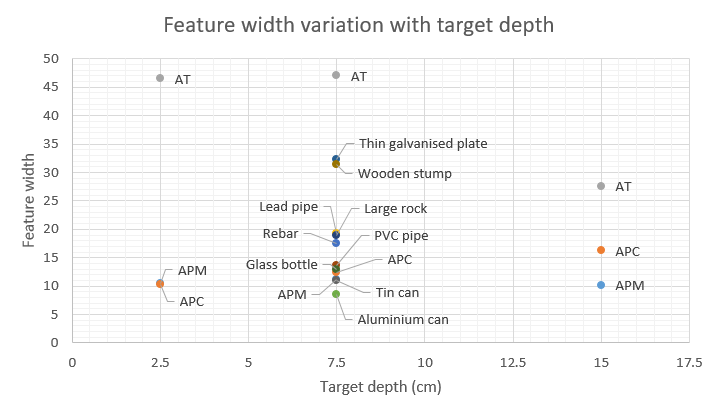
\includegraphics[width=\textwidth]{5-Testing/featureWidth.PNG}
\centering
\caption{Feature width variation with target depth}
\figlabel{featureWidth}
\end{figure}

The results for the feature depth (\Figref{featureDepth}) are quite similar to the feature width at the target depth of 7.5cm. The characteristics and false positive rates are high for both APC and AT where the feature depth was similar to that of a large rock. However, this percentage probability can be differentiated using the feature width metric. Similarly, the feature width false detections for the tin can, glass bottle and PVC pipe can be differentiated using the feature depth.  The APM is distinguishable for all three depths for this plot.

\begin{figure}[!ht]
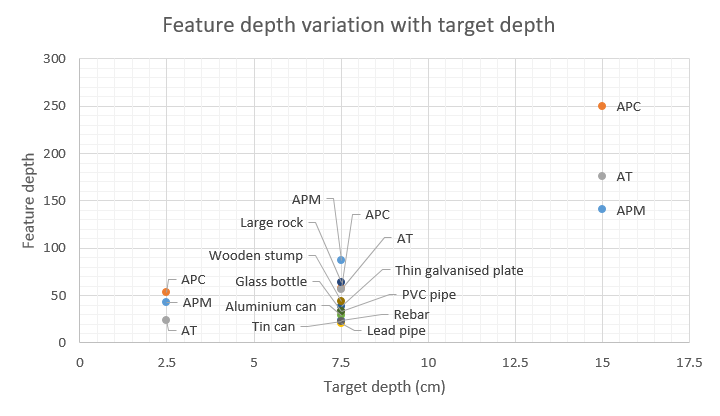
\includegraphics[width=\textwidth]{5-Testing/featureDepth.PNG}
\centering
\caption{Feature depth variation with target depth}
\figlabel{featureDepth}
\end{figure}

When feature depth is plotted against the variation of feature width, all three mines have distinguishable features, with no clutter within their calculated ranges (\Figref{depthWidth}). Although it is differentiable, the clutter objects (aluminium can, tin can, glass bottle and PVC pipe) were found to be within close proximity to the signatures of both APM and APC at shallow target depths of 2.5 cm and 7.5 cm.

\begin{figure}[!ht]
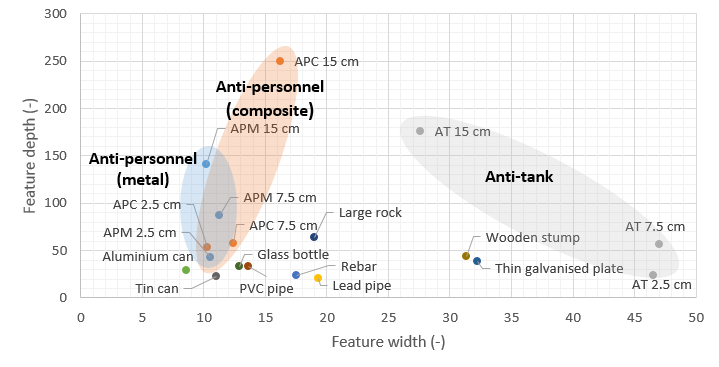
\includegraphics[width=\textwidth]{5-Testing/depthWidth.PNG}
\centering
\caption{Feature depth variation with feature width}
\figlabel{depthWidth}
\end{figure}

The results from the plots in previous pages can be summarised in the table below \Tabref{gprMetrics}. The AT is both distinguishable at all target depths using the feature width metric, and APM is distinguishable using the feature depth metric. As shown, the feature width has the lower percentage confidence at 73\%, with three objects (PVC pipe, glass bottle and tin can) out of eleven detected as an APC or APM. In comparison, the feature depth only produced one false positive, the large rock scanned as shown in \Tabref{gprMetrics}, out of the eleven objects scanned, which gives a 90\% confidence. From these results, the percentage confidence and objects can be confirmed without the use of metal detector metrics. 

\begin{table}[!ht]
\centering
\caption{Summary of the false positive detection for GPR metrics}
\tablabel{gprMetrics}
\begin{tabular}{lll}
\toprule
Object & Feature width & Feature depth \\ \midrule
All APM & APM/\textbf{APC} & APM \\
All AT & AT & AT/\textbf{APC} \\
All APC & APC/\textbf{APM} & APC/\textbf{AT} \\
Thin galvanised plate & Thin galvanised plate/Wood & Thin galvanised plate \\
Wood & Wood/Thin galvanised plate & Wood \\
Rock & Rock/Lead pipe & \textbf{APC/AT} \\
PVC pipe & \textbf{APC} & PVC pipe \\
Glass bottle & \textbf{APC} & Glass bottle \\
Tin can & \textbf{APM} & Tin can/Lead pipe \\
Aluminium can & Aluminium can & Aluminium can/PVC/Rebar \\
Rebar & Rebar & Rebar/PVC/Aluminium can \\
Lead pipe & Lead pipe/Rock & Lead pipe/Tin can\\ \bottomrule
\end{tabular}
\end{table}

\subsubsection{Discussion}
The results show that the algorithm can produce unique sets of data and is able to distinguish between the landmines and clutter objects. The metal detector output metrics produced consistent results and identified the AT and APM mines from both tests. In comparison, the GPR was able to distinguish between both metallic and non metallic objects, however, it was not as consistent as the metal detector output metrics and, therefore, produced a higher rate of false positives.

\textcolor{blue}{Although data has been consistent, there were limitations to this data that require further work, such as, burying objects at 2.5 cm and 15 cm similar to the dummy landmines. This will enable better comparison due to the larger data set and because it will show whether there is a higher or lower false positive rate at the different depths for the clutter objects. \\
Another limitation for this data is that it cannot be replicated for other soil types as there is a difference between sensor signals when objects are placed in this type of soil. This may be due to a number of factors, such as inconsistencies with soil, other ground objects and moisture content. The moisture content of the soil may have affected results as the tests were completed after heavy rainfall and it was calculated to have approximately 20\% moisture. \\
Further tests may be completed in a controlled environment to enable change to the object's orientation, type of soil and moisture control. This will enable further comparison of these effects on the signals and false positive reduction. Hence, it will also enable an improved algorithm design by making it more dynamic according to the differences in environment and other inputs. 
}

Regardless, the false positives can be reduced when the results from both sensors are combined using the sensor fusion algorithm discussed in detailed design.

%%%%%%%%%%%%%%%%%%%%%%%%%%%
\todo[inline]{Some points are here, as you said, the other stuff can be in future design, need to check if }
%%%%%%%%%%%%%%%%%%%%%%%%%%%

\textcolor{red}{Seems to be some repetition here from the detailed design for sensor fusion. Need to discuss what some of the limitations of the tests were. Only a small number of clutter objects were used, clutter was only buried at one depth, if it was some other depth is might have led to more/less false positives, i.e. the current data set needs to be expanded on largely in order to make the detection algorithm more robust. The same type object would have a different signature if it was a different size, or in a different orientation - need to do more sensitivity testing, ideally in a controlled environment with the use of a test rig, allowing for repeated sweeps in an identical manner. \textbf{Some of these points could go in future work.}The results can't really be applied to any other scenarios, as both metal detector and GPR signals will look different in different soil types. Soil moisture was high, and the soil wasn't very clean (not layered nicely, rocks and things present), this may have had an effect on GPR results.Would be better to test in DSTG test lanes. Could not achieve real time processing, however the sensor fusion algorithm (still needs to be done) was tested with sample data to simulate batch processing of results.}

\section{Quad bike systems testing}
Preliminary testing of the quad bike subsystems were required to determine their working range, functionalities and integration. The systems tested were the brakes, steering, throttle, gear selector, wheel encoder, and positioning system. Additional safety systems were also tested to ensure they functioned as intended.
The relevant test objectives and test cases were documented and can be found in (\textcolor{red}{ APPENDIXXX}).
\todo[inline]{add hte corect appendix here}

\subsection{Brake testing}
The brakes were required to control the quad bike speed as well as to bring the platform to a complete stop when commanded to or in the case of an emergency which is important to the project goal. This requires accurate knowledge of the brake position for the varying brake intensities. The objectives for the braking test were to:

\begin{enumerate}
\item Determine required braking intensity to stop the wheel spinning and the required retraction to spin the wheel freely again
\item Determine duration required for brake activation
\item Determine braking distance to come to a complete stop from operational speed  
\end{enumerate}

The brakes are important to the project goal as they have the ability to make the platform safe and controllable. Without them the platform would be slow to stop potentially putting personnel in close proximities to it in danger.

The maximum brake intensity was chosen as the point where the wheels were unable to be turned by hand. This was found through small 5 percent increments in the actuator extension until the wheels were unable to rotate. This was selected as the 100\% braking intensity and the point where the wheels spun freely chosen as the 0\% braking intensity. The linear transducer outputs values from 0 for fully retracted to 1023 for fully extended. The 0\% and 100\% braking intensities were mapped to transducer values of 435 and 660, respectively.

The time required for the brake actuator to go from the chosen zero brake position to the 100 \% was measured to be 2.4 seconds. Travelling at 5 km/h, the time delay would result in the quad bike being unable to come to a complete stop in the required distance. %An attempt to counteract the 2 second braking time was to couple this with a reduction in throttle. As the quad bike would still be in gear, the gearing and engine would act as an engine brake potentially stopping the quad bike sooner. 
%\todo[inline]{is this sound logic?}

During testing, it was found that the throttle response was much faster in operational response and did benefit in the braking distance. Strategic braking locations were implemented into the navigation software to ensure that the path traversed was accurate. However, if the quad bike were to detect a landmine, there would be no time for the sensors and the throttle to slow the bike down in time. An overshoot of the desired stopping point was approximately 1 meter (see \secref{liveplatformnavigation}).

The brake speed and thus actuator choice were insufficient for the required task and only proved useful in holding the position of the bike during navigation manoeuvres. With only engine braking, the quad was found to coast to a stop from operating speeds in 1.2 m. With the brakes activating, the quad bike was able to come to a complete stop in 1 meter. This exceeds the platform requirements resulting in the need for a faster brake actuator. A deluxe rod actuator type FA-HF-100-12-9" from Firgelli Automations is the recommended part for any future use. It provides similar dynamic force capabilities, 444 N compared with 578 N, and much faster actuator speeds, 76 mm/s compared with 12 mm/s. This actuator would take 0.4 seconds to engage the brake from 0 to 100\% intensity. At an operational speed of 5 km/hr the quad bike would stop in 0.5 meters.

\subsection{Gear testing}
The ability to control what gear the quad bike is in was essential to the control and navigation of the project. 36 testing cases were identified for the gear actuator setup. The actuator could lie in one of nine possible positions (\Figref{gearPositions}) which were identified based on the system set-up and had three possible final positions to move to, reverse, neutral and forwards as well as a null option for no actuator movement. 
\begin{figure}[ht]
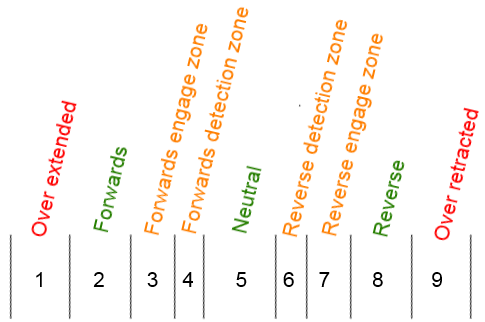
\includegraphics[width=0.6\textwidth]{5-Testing/gearDiagram.png}
\centering
\caption[Gear positions]{Gear positions}
\figlabel{gearPositions}
\end{figure}
\Chapref{gearTable} shows the final truth table. The gear actuator completed each of the 36 test cases. A number of safety checks were also implemented into the movement. The gear actuator should not move when the quad bike is in motion or when the throttle is engaged. This is to ensure that control of the quad bike gearing system is maintained at all times.  A check in the software was implemented to achieve this. Testing of the system resulted in fine tuning requirements of the gear position sensors. Initial tests resulted in the gear not mechanically being inserted even if it displayed it had on the quad bike display. This resulted in gearbox cogs grinding and the quad bike lurching forwards when the gear caught. Further tests lead to the adjustments in the Quad bike idle throttle position. Due to the idle being set too high, the centrifugal clutch would engage before the gear was properly selected leading to more gearbox grinding. Proper idle speeds resulted in smooth gear changes with no lurching or gearbox grinding.

\subsection{Steering testing}
The steering of the quad bike was achieved through the use of a stepper motor. Upon power up, the position of the wheels would be the zero position and movement to the left or right was dictated by the angle sent to the stepper motor. From the user manual for the quad bike the lock out angle for the steering was 24 degrees, a limit for the steering angle was placed at 23 degrees to ensure no accidental structural damage occurred.

Initial tests found that when the quad bike was on the support stand with the wheels free, the steering behaved as expected. However, when a resistive load was applied in the direction of the steering angle, the stepper motor would stop and reset. This would result in an incomplete steering angle as well as a new off centre zero position being selected by the stepper motor.  It was found that the required power for the stepper motor to operate to the required torque was 440 W whereas the power supply in the quad bike was only able to supply 44 W. This meant that under moderate loads the power supply couldn't supply the required current and failed. Replacement of the power supply with one of the correct power requirements resulted in steering angle control under operational loads.

The accurate turning radius for the platform was required for the navigation software. The quad bike was allowed to travel in both forwards and reverse from a marked position with the steering at full lock. Once a half circle was complete, the quad bike was turned off. Initial tests were completed by manually pushing the quad bike and follow up tests completed with the quad bike under its own power. The test results are summarised in \tabref{turnRadiusTests}. Manual turns achieved tighter turning circles caused due to human bias towards the turning direction. The powered tests had larger turn circles due to some skidding on the turning wheels. The turning radii experienced were within the turning circle range decided upon in the navigation software.
\begin{table}[ht]
\centering
\caption{Steering turn radius tests}
\tablabel{turnRadiusTests}
\begin{tabular}{ll}
\toprule
Test & Turn circle radius \\ \midrule
Manual forwards & 2.7 \\
Manual reverse & 3.2 \\
Powered forwards & 3.0 \\
Powered reverse & 3.5 \\ \bottomrule
\end{tabular}
\end{table}

\subsection{Throttle testing}
The throttle is controlled via a rotational servo. Initial approximation of the throttle travel had the servo with zero throttle and maximum throttle at servo positions 75 and 150 respectively. With the engine warmed up, incremental increases resulted in an actual throttle response range to be calculated. Due to the circular sweep of the servo arm and some cable play, the minimum throttle position before a throttle response was found to be 97 and a maximum throttle position of 110 was chosen for the servo. This number was chosen due to the wheel speed in both forwards and reverse gears varying due to gearing and so the maximum servo position would be required for cruise speed in both directions of motion. A higher servo position than this would never be required for the chosen operating scenario.

live tests on the ground found that the added load on the drive-train only resulted in the quad bike moving forward when the throttle was set to 70\% of the selected range of motion. once the quad bike started moving forwards and at operational speeds, a throttle of 60\% was required to maintain the speed. Different terrains would offer different drag coefficients on the wheels leading to different throttle responses to overcome the initial drag to get the quad bike in motion.

\section{Positioning systems testing}
Knowing the error distribution accurately is an important part of the Kalman Filter and is why it is able to output a very reliable position estimate. Each positioning system was tested and their errors analysed to be used in with Kalman Filter. 
\subsection{GPS}
The primary function of the GPS in the positioning system was to correct for drift that may be present in the kinematic equations. For this purpose accuracy is very important however very small emphasis is placed on any error from noise, which is accounted for in the Kalman Filter. Testing of the GPS involved moving it around a known location over known distances. Two categories of testing were conducted, stationary tests and non-stationary tests. This was chosen as a result of the known differences in performance between the two.
\begin{figure}[ht]
\centerline{
\begin{tabular}{cc}
\subfloat[Non-stationary test]{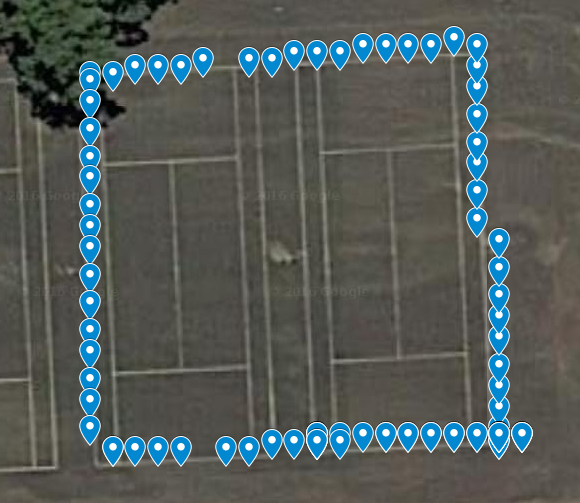
\includegraphics[height=0.4\textwidth]{5-Testing/nonStationaryGpsTest.png}} 
& \subfloat[Stationary test]{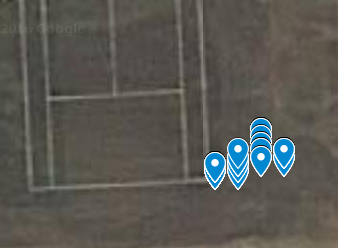
\includegraphics[height=0.4\textwidth]{5-Testing/stationaryGpsTest.png}}\\
\end{tabular}}
\caption{GPS tests}
\figlabel{gpsTests}
\end{figure}
The non-stationary test in \Figref{gpsTests}a involved traversing the outer edge of two tennis courts, and during the stationary test in \Figref{gpsTests}b the receiver was left sitting in the bottom right corner of the tennis court for 120 seconds. The GPS data was overlayed onto satellite imagery using Google Maps for better visualisation.

From the non-stationary test it is evident that when moving the GPS provides very accurate positional information, within 1 meters for the duration of the test. The stationary test revealed that the GPS suffers quite substantially from drift when sitting still, varying up to 6 meters from its actual position. For this reason, the GPS will only be to correct positional information in the Kalman Filter when the quad bike is at cruising speed, 5 km/hr.

\subsection{IMU}
To determine error present in the IMU it was correctly set on the quad bike and the engine started and throttled. The test procedure allowed the IMU to calibrate for 35 seconds before starting the engine. The engine idled for 45 seconds, then was throttled for 40 seconds before being turned off. The results are shown in \Figref{yawTest} and \Figref{yawTestZoomed}.
\begin{figure}[ht]
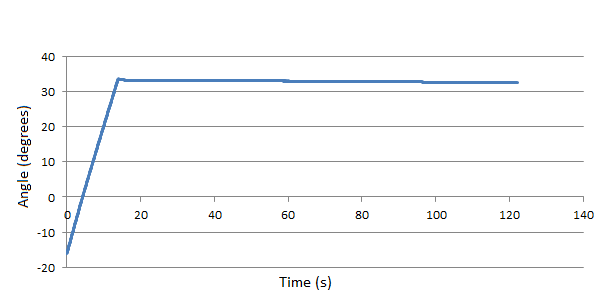
\includegraphics[width=1\textwidth]{5-Testing/yawTest.png}
\centering
\caption{Yaw test: calibration to 35 s, idle to 80 s, throttle to 120 s}
\figlabel{yawTest}
\end{figure}
\begin{figure}[ht]
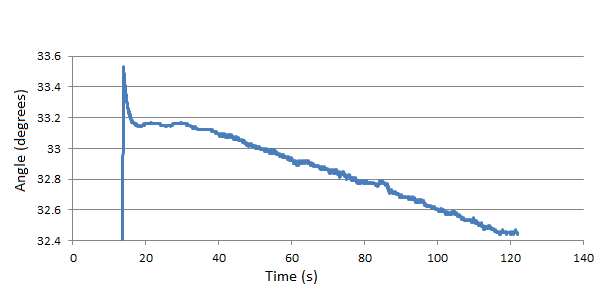
\includegraphics[width=1\textwidth]{5-Testing/yawTestZoomed.png}
\centering
\caption{Yaw test focused on angle from 32.4\degree to 33.6\degree}
\figlabel{yawTestZoomed}
\end{figure}
The IMU takes some time to calibrate, we can see from \Figref{yawTestZoomed} that calibration is complete at $t=20s$. Over the remaining 15 seconds before the engine is started, the IMU holds its position almost perfectly. Over the remaining 85 seconds of the testing period, the IMU heading steadily decreases by a total angle of 0.7 degrees, a rate of $\frac{0.7\degree}{85\ seconds} = 0.008 \degree/s$. The same slope between idling and throttling showed that the error of the IMU did not depend on the rate of throttle of the engine, just if the engine was running or not.

Raw accuracy of the IMU was found by smoothly rotating the IMU 360\degree on a desk. Initial IMU readings were 87.3 degrees and the reading after the rotation was \~85.6 degrees, an error of $\frac{2\degree}{360\degree}$, or $0.056\degree/\degree$. When used in the Kalman Filter the errors are factored either by the time step or the rotation angle of the IMU.

\subsection{Wheel encoder}
\seclabel{testingwheelencoder}
One of the primary functions of the wheel encoder was to give an accurate value for the distance travelled by the quad bike as well as it's operating speed for use in the kinematic equations of the Kalman Filter. To test the encoder, data was compared with values obtained from the display unit on the quad bike. The two data sets are overlaid in \Figref{encoder20x} and the instantaneous difference shown. Some sampling was necessary to reduce the noise present in the encoder data. 20x was found to be the best as it was able to smooth the noise while keeping accurate to the display speed. It was clear that the wheel encoder was doing an adequate job of representing the display speed. The second test was to evaluate how accurate the speed represented the actual distance travelled when integrated over time. \Tabref{encoderIntegration} shows the results of three tests. Test 1 and 2 consisted of manually spinning 10 revolutions of the quad bike wheel on its stand at a consistent speed. Test 3 involved 3 complete stops of the wheel throughout the 10 revolutions. The errors from this test were used in the Kalman Filter.

\begin{figure}[ht]
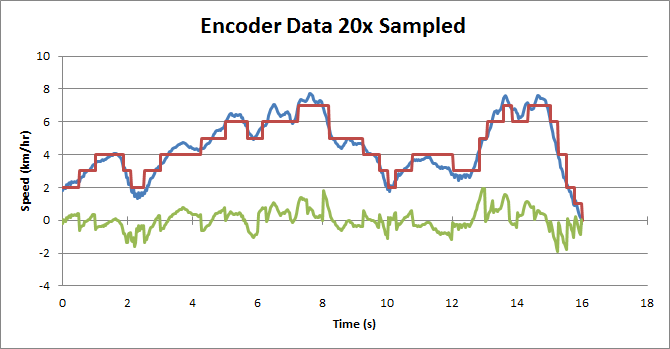
\includegraphics[width=1\textwidth]{5-Testing/encoder_data_20x_sampled.png}
\centering
\caption[Encoder speed reading compared with quad bike display]{Encoder speed reading compared with quad bike display with engine not running}
\figlabel{encoder20x}
\end{figure}

\begin{table}[ht]
\centering
\caption{Wheel encoder distance integration tests}
\tablabel{encoderIntegration}
\begin{tabular}{llll}
\toprule
                                   & Test 1 & Test 2 & Test 3 \\ \midrule
Rotations of the wheel:            & 10     & 10     & 10     \\
Number of readings:                & 7646   & 8843   & 19885  \\
Test time (seconds):               & 13.54  & 14.39  & 31.69  \\
Time interval (microseconds):      & 1770   & 1627   & 1594   \\
Circumference of wheel (m):        & 1.95   & 1.95   & 1.95   \\
Actual distance travelled (m):     & 19.5   & 19.5   & 19.5   \\
Calculated distance travelled (m): & 19.53  & 19.41  & 18.86  \\ \bottomrule
\end{tabular}
\end{table}

Tests for the encoder with the quad bike engine running were completed to see if the operation of the engine effected the speed output. \Figref{encoderEngine} shows the encoder readout for the engine tests. It can clearly be seen that there are large discrepancies in the speed outputs. It was found that the encoder support bracket vibrated against the encoder wheel resulting in large spikes in the speed reading. Upon firmly supporting the bracket, the noise was reduced but still present. A rubber damper and a support bracket was fixed to the encoder support and this reduced the noise level. However the reduction was still not adequate for the required accuracy. 

Speed tests were completed with the quad bike moving under its own power. The encoder readings were accurate however, large fluctuations were still inherent. A low pass filter was used to smooth out the data from the encoder leading to smoother and more accurate speed readings from the encoder. However, at idle the encoder still read incorrect velocities that could not be eliminated by the low pass filter. The main consequence of the velocity reading fluctuations was with the navigational software. Due to incorrect velocity readings at zero speed, the navigation software placed the quad bike at a position that was inaccurate.

\begin{figure}[ht]
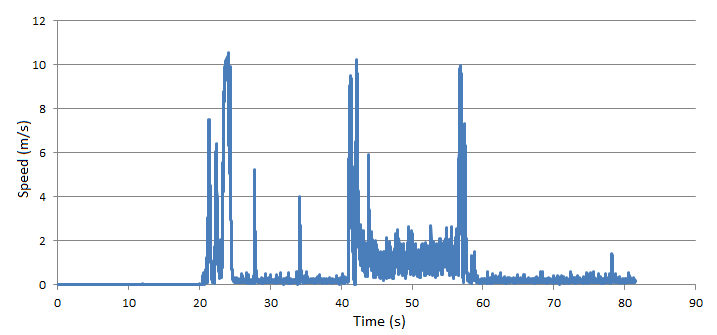
\includegraphics[width=1\textwidth]{5-Testing/Encoder_data_with_engine_running.png}
\centering
\caption[Encoder speed reading for various engine states]{Encoder speed reading when stationary and engine off (0s - 20s), engine idling (20s - 40s), engine throttling (40s - 60s), and while supporting the encoder bracket (60s - 80s)}
\figlabel{encoderEngine}
\end{figure}

\subsection{Integrated positioning system}
Testing for the positioning system was primarily undertaken inside the Virtual Platform (see \secref{detailedVP}). This was to ensure satisfactory performance of the system before live tests were undertaken. Simulated hardware components; GPS, IMU, and wheel the encoder, were used inside the Virtual Platform. Noise for each of the sensors was hard-coded into the software based on the values obtained from their respective tests.
\Figref{posError1} shows the x and y components of the distance error from the true value for the Kalman filtered position and the position from kinematic equations for comparison. The simulation consisted of a 25 degree right turn, 25 degree left turn, followed by a long straight beginning at the nine second mark. Due to the certain starting position of the quad bike the errors all begin at zero. When using the kinematic equations alone, the error grows due to the additive nature of the process. A diverging result occurs because the heading calculated through kinematics is not the true heading. When corrected with the IMU and GPS the Kalman position stabilises and the error peaks at approximately 0.4 meters, which is within specifications. \Figref{posError2} is a more realistic simulation, consisting of 2 x 90 degree right turns, a long straight, and 2 x 90 degree left turns to mimic a path that would be traversed throughout a set region. It is again apparent with the kinematic equations alone that error accumulates when a straight is encountered. When stabilised with the IMU and GPS units however, the resulting Kalman position remains accurate to within 0.2 meters, again within specifications.
\begin{figure}[ht]
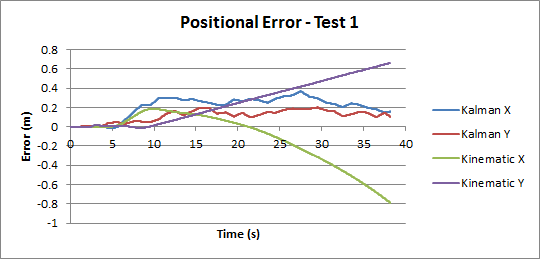
\includegraphics[width=\textwidth]{5-Testing/position_error_test_1.png}
\centering
\caption[Positioning system test 1]{Test 1: 25 degree right turn, 25 degree left turn, followed by long straight (from 9 seconds)}
\figlabel{posError1}
\end{figure}
\begin{figure}[ht]
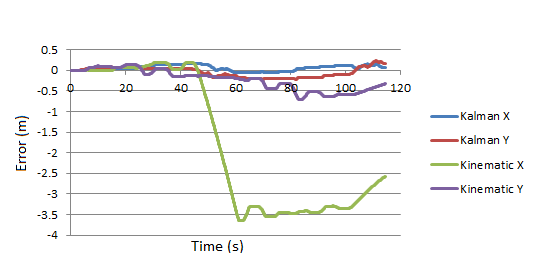
\includegraphics[width=\textwidth]{5-Testing/position_error_test_2.png}
\centering
\caption[Positioning system test 2]{Test 2: 2 x 90 degree right, long straight, 2 x 90 degree left, long straight} \figlabel{posError2}
\end{figure}

\section{Navigation testing}
\subsection{Virtual platform}
All navigation was initially 
\todo[inline]{finish this section harry you fucking bastard!}

\subsection{Live platform}
\seclabel{liveplatformnavigation}
Navigation testing consisted of a series or predefined routes that the quad bike would have to traverse autonomously. The objectives of the testing was to determine the following:

\begin{enumerate}
\item Accuracy of the wheel encoder for distance calculations as the distance traversed calculated via the wheel encoder was heavily relied upon in the positioning software and hence navigation software.
\item Turn angle accuracy from the set path to the actual platform under operating conditions. 
\item Path following ability of the real platform compared with an on screen representation of where the positioning system estimates the real quad bike position.
\end{enumerate}

In order for these objectives to be tested for, test cases were generated. These test cases described the various tests utilised in order to deem the completion of the assigned objectives. The test cases included straight line travel over a set distance and stopping at a set point, simple turns through a range of angles up to complex turns andfinally a right angle turn.
 
Each test starting point was marked with a flag. The key points throughout the designated path were also marked with flags to ensure that the correct actions where being carried out by the quad bike in the correct locations. This was done to examine the path of the quad bike with the ideal path mapped by the navigation software.

The initial straight line test was used to find the stopping distance and necessary throttle and actuator inputs to result in the desired distance travelled. The most important outcome of this test was to match the real quad bike position with the estimated quad bike position as displayed on screen. Minor factor modifications were made to the applied throttle, time of throttle, look ahead distance and wheel encoder output.

Simple turns starting from 20 degrees were then completed. It was found that due to the added resistance from the dragging steering wheels, the throttle would be required to be increased. Due to the added drag, the actual turning angles varied from the positioning software which resulted in reduced angles of turn. This was because the positioning estimation would complete the required turn angle and command a different steering angle before the real quad bike had achieved the initial desired turn angle. This become more evident during the complex turns as the turn angles became more and more reduced for each increasing test angle.

\todo[inline]{harry will add more here about how good the test went!!! ie. stuff about hte actuators all functioning correctly and at the correct times etc. etc. also a diagram of each of the tests}

Further testing should be conducted on larger test courses so the GPS and IMU are able to have some measurable impact on the positioning software.

\end{document}